%%%% 1. DOCUMENTCLASS %%%%
\documentclass[journal=tosc,final]{iacrtrans}
%%%% NOTES:
% - Change "journal=tosc" to "journal=tches" if needed
% - Change "submission" to "final" for final version
% - Add "spthm" for LNCS-like theorems


%%%% 2. PACKAGES %%%tsdss
\usepackage[left, pagewise,edtable]{lineno}
\usepackage{blt}
\usepackage{graphicx}
\usepackage{framed} 
\usepackage{xcolor}
\usepackage{tcolorbox}
\usepackage{xcolor} 
\usepackage{listings}
\usepackage{quoting} %
\colorlet{shadecolor}{gray!25}
\definecolor{mshadecolor}{rgb}{0.7421875,0.7421875,0.7421875}
\setlength{\OuterFrameSep}{10pt}
%%%% 3. AUTHOR, INSTITUTE %%%
\author{Moritz Rupp}
\institute{
  Hochschule Albstadt-Sigmaringen, Albstadt, Germany, \email{ruppmori@hs-albsig.de}
  
}



%%%% 4. TITLE %%%%
\title{Soziotechnische Lösungsansätze gegen Phishing}

\author{Moritz Rupp}

\begin{document}

\maketitle
\author

\begin{center}
\date{Sommersemester 2023 } 
\end{center}



%\vspace{15mm}
%%% 5. KEYWORDS %%%%s
\keywords{Social-Engineering \and Phishing \and IT-Security \and Container \and DNS }


%%%% 6. ABSTRACT %%%%s
\begin{abstract} Phishing zählt nach wie vor zu den häufigsten Methoden bei Cyberangriffen. Dabei werden versucht vertrauliche Informationen wie Passwörter oder Kreditkartennummern abzugreifen. Hierbei werden soziale Manipulationstechniken oder gefälschte Kommunikationskanäle genutzt, um das Vertrauen des Opfers zu gewinnen. Diese Arbeit untersucht Technische Lösungsansätze um dies vorzubeugen.  \end{abstract}

\newpage
\tableofcontents
\newpage

%%%% 7. PAPER CONTENT %%%%
\section{Einführung}
Phishing ist eine Form des betrügerischen Verhaltens im Internet, bei der Angreifer versuchen, sensible Informationen wie Benutzernamen, Passwörter, Kreditkartennummern oder andere persönliche Daten von Internetnutzern zu stehlen. Dies wird bewerkstelligt, indem Angreifer gefälschte Webseiten, E-Mails oder andere Kommunikationskanäle nutzen, um sich als vertrauenswürdige Quellen oder Organisationen auszugeben. Das Hauptziel des Phishings besteht immer darin, Opfer zu verleiten, ihre vertraulichen Informationen preiszugeben, indem sie beispielsweise auf einen gefälschten Link klicken, ihre Anmeldedaten auf einer gefälschten Website eingeben oder auf betrügerische E-Mails antworten.

Dazu nutzen Phishing-Angriffe oft soziale Manipulationstechniken, um das Vertrauen der Opfer zu gewinnen. Dies kann beispielsweise durch die Nachahmung von bekannten Unternehmen, Regierungsbehörden oder Finanzinstituten erfolgen. Die Angreifer verwenden entsprechende Sprache, gefälschte Logos und weitere Taktiken, um ihre gefälschten Kommunikationen authentisch wirken zu lassen.

Ein erfolgreicher Phishingangriff hat schwerwiegende Konsequenzen für die Opfer. Durch den Diebstahl persönlicher Daten können die Angreifer Identitätsdiebstahl begehen, finanziellen Schaden anrichten oder die gestohlenen Informationen für weitere kriminelle Aktivitäten nutzen. Darüber hinaus kann Phishing das Vertrauen der Benutzer in Online-Dienste und elektronische Kommunikation insgesamt untergraben.

Die Bekämpfung von Phishing erfordert eine Kombination aus technischen Lösungen, Benutzererziehung und rechtlichen Maßnahmen. Dies umfasst beispielsweise die Implementierung von Sicherheitsprotokollen wie E-Mail-Authentifizierung, Anti-Phishing-Filtern und Phishing-Warnungen in Webbrowsern. Die Sensibilisierung der Benutzer für Phishing-Techniken und die Förderung bewusster Online-Sicherheitspraktiken spielen ebenfalls eine wichtige Rolle bei der Verringerung des Risikos von Phishing-Angriffen.\\ Die Kombination von technischen und sozialen Komponenten und deren Abhängikeiten, kann als Sozio-technisches System bezeichnet werden. Die Strukturierung bzw. Beschreibung von solch einem System im Context von Phishing, kann hilfreich sein um die komplexe Landschaft aus Angriffvektoren und Präventivmaßnahmen richtig einordnen zu können. Diese Arbeit behandelt Sozio-technische Systeme  als Lösungsansatz gegen Phishing Angriffe. Dafür wird im ersten Schritt ein Sozio-technisches System definiert und auf Phishing angewand. Anschließend werden die teilkomponenten wie soziale und technische Lösungen vorgestellt und abschließend als gesamte Lösung zusammengeführt. 


\newpage

\section{Soziotechnische Systeme}
Ein soziotechnisches System ist ein Konzept, das die Wechselwirkung zwischen sozialen und technologischen Elementen in einer bestimmten Umgebung oder Organisation beschreibt. Konkret wird die Tatsache betrachtet, dass in vielen Bereichen und Systemen ein Zusammenspiel sowie eine Abhängigkeit zwischen Menschen und Technologien besteht. Zudem wird festgestellt das die Implementierung von Technologien nicht isoliert von sozialen, kulturellen oder organisatorschen Aspekten betrachtet werden kann. Stattdessen besteht selbst in vermeintlich rein technologischen Prozessen immer eine Abhängigkeit von Menschlichen, irrationalen Einflüssen. Dies ist Grundbestandteil eines Soziotechnischen Systems. Die Teilsysteme sind voneinander nicht trennbar, sondern es bestehen verschieden ausgeformte Abhängigkeiten.\\
Es ist möglich nahezu alle adaptiven Systeme als Soziotechnische Systeme zu modellieren. Darunter fallen beispielsweise Flugkontrollsysteme, Social-Media Plattformen, Krankenhausinformationssysteme oder Bildungseinrichtungen.\\
In Figure 1 wird ein Arbeitssystem als Soziotechnisches System dargestellt.
\begin{figure}[h]
\caption{Soziotechnisches System}
\begin{center}
 \includegraphics[scale=0.5]{sozio.png}
\end{center}
\end{figure}

Generell besteht ein Soziotechnisches System aus 2 Grundkomponenten.. Einer technische Teilkomponente und einer soziale Teilkomponente. Diese haben jeweils weitere Subkomponenten. Das Arbeitssystem besteht aus 2 sozialen Teilkomponenten. Mitgliedern sowie Rollen bzw. Strukturen. Zudem gibt es 2 Technische Teilkomponenten. Eine Technologie, und eine definierte Aufgabe. Alle Teile des Arbeitssystems haben Abhängigkeiten untereinander. Um nun aus einem Input einen Output zu erzeugen, müssen alle Teilkomponenten wechselseitig Interagieren. Fällt eines der Teilkomponenten aus, so ist das gesamte Arbeitssystem nicht mehr lauffähig. Die Technologie bearbeitet und verbessert die Arbeitsprozesse, während die Mitarbeiter ihr Fachwissen und ihre Erfahrung einbringen, um die Systeme zu steuern, zu überwachen und anzupassen. Die Effizienz und Qualität der Produktion hängen sowohl von der technischen Leistungsfähigkeit als auch von der Zusammenarbeit und Interaktion zwischen den Menschen und der Technologie ab. Die Betrachtung von Soziotechnischen Systemen ist wichtig, um die Auswirkungen technologischer Veränderungen auf die Arbeitswelt, die Gesellschaft und die Menschen zu verstehen. Es fördert einen ganzheitlichen Ansatz bei der Gestaltung und Implementierung von Technologie, bei dem soziale, organisatorische und technologische Faktoren berücksichtigt werden, um positive Ergebnisse und ein besseres Zusammenwirken von Mensch und Technologie zu erzielen. Insbesondere kann es helfen Problematiken in komplexen Systemen und Prozessen zu verstehen und richtig einzuordnen. Davon ausgehend können nun Lösungen entwickelt werden, die sowohl technische als auch soziale Aspekte miteinbeziehen.  
\newpage
\subsection{Phishing als Soziotechnisches System}
Ein Phishingangriff kann als ein Soziotechechnisches System modelliert werden. Die technischen Komponenten umfassen den Einsatz von Webseiten, E-Mails oder Kurznachrichtendiensten. Zu sozialen Komponenten zählen Angreifer sowie die Phishing Opfer. Des weiteren gibt es zwischen technischen und sozialen Komponenten Interaktionen und Abhängigkeiten. Um ein vollständiges System zu modellieren, muss zudem ein Ziel definiert werden. In Figure 2 ist Phishing als Soziotechnisches System modelliert.
\begin{center}
 \begin{figure}[h]
  \caption{Phishing als Soziotechnisches System}
  \includegraphics[scale=0.5]{syst.png}
 \end{figure}
\end{center}
Hierbei spielen die technischen Subkomponenten wie Webseiten, E-Mails und Messenger Dienste, wechselseitig mit den sozialen Subkomponenten wie Anreifer und Opfer zusammen, um an das Ziel, in Form von Informationen und Geld zu gelangen. Genauer  betrachtet bedient und missbraucht ein Phishingangriff die verschiedenen Komponenten. 

\begin{enumerate}
\item Technische Komponenten
\begin{itemize}
\item Mail-Server: Der Server, über den Phishing-E-Mails an potenzielle Opfer gesendet werden.
\item Phishing-Website: Eine gefälschte Website, die erstellt wurde, um die Opfer zur Preisgabe ihrer vertraulichen Informationen zu verleiten.
\item DNS-Server: Der Server, der die Domainnamen auflöst und es den Angreifern ermöglicht, gefälschte Domains zu verwenden.
\end{itemize}
\item Soziale Komponenten
\begin{itemize}
\item Phisher: Die Angreifer, welche die Phishing-Angriffe initiieren.
\item Opfer: Die Personen, die das Ziel der Phishing-Angriffe sind.
\end{itemize}
\end{enumerate}
Die Interaktion zwischen diesen Teilkomponenten sind beispielsweise der E-Mail Versand, die Nutzung von Webseiten oder die Preisgabe von Informationen. Diese Modellierung zeigt, die starke Interaktion zwischen den Komponenten. Zudem können Schwachstellen in diesem System identifiziert werden und geeignete Schutzmaßnahmen implementiert werden.
\subsection{Phishing-Prävention}
Durch die Betrachtung von Phishing als Soziotechechnische System, ist festzustellen das dieses eine hohe Anzahl an Abhängikeiten aufweist. Wir wir wissen, sind die Teilsysteme nicht voneinander trennbar. Fällt eines der Subkomponenten aus, stoppt der Arbeitsprozess in Form des Phishing Angriffes. Wäre es möglich eines oder mehrere der Subkomponenten vollständig  abzuschalten, könnte der Wirkungsgrad eines Phishingangriffes stark eingegrenzt werden. Dies gilt insbesondere für die Nutzung der Technischen Komponenten von seiten des Opfers. Diese werden als Einstiegskanal für die Interaktion zwischen Angreifer und Opfer genutzt. Könnte man also konkret die technische Teilkomponente wie ein E-Mail Client isolieren, wäre eine Interaktion deutlich schwerer. Auch Soziale Komponenten können verwendet  werden um einen Phishingangriff zu unterbinden. Die Effectivste Methode besteht jedoch darin, soziale und technische Teilkomponenten in einer soziotechnischen Lösung zusammenzuführen.
\section{Soziale Lösungsansätze}
Soziale Lösungsansätze gegen Phishing konzentrieren sich auf die Stärkung der Benutzer, die Sensibilisierung der Öffentlichkeit und die Organisation von Richtlinien.\\
Durch Schulungen, Workshops und Informationskampagnen können Benutzer über Phishing-Techniken, Angriffsvektoren und typische Warnsignale aufgeklärt werden. Ziel sollte es sein zu lernen, verdächtige E-Mails zu identifizieren, Links und Anhänge zu überprüfen und verschiede Phishing-Angriffen zu erkennen. Dies beinhaltet das Erlernen von Indikatoren wie Grammatik- und Rechtschreibfehler, verdächtige URLs, Anfragen nach persönlichen Informationen oder Finanzdaten und die Nutzung von Social Engineering-Taktiken. Zudem sollte auch über die verschiedenen Arten von Phishing informiert werden, wie z. B. Spear-Phishing, Pharming und Vishing.\\ Um die Kompetenzen der Nuutzer weiter zu stärken, können praktische Übungen und Phishing-Simulationen durchgeführt werden. Hierbei werden  Phishing-E-Mails oder gefälschte Websites präsentiert, um die Fähigkeit der Nutzer zur Erkennung und Handhabung von Phishing-Angriffen zu testen. Zudem sollten spezielle Programme für nicht IT-Affine Nutzer bereitgestellt werden. Eine Studie fand heraus das Wissen über Phishingangriffe stark altersabhängig ist. Hierbei wurden vier Altersgruppen zwischen 18 bis 55 Jahren zu Terminologie von Phishing befragt. Personen ab 55 Jahren waren die Begriffe „Phishing“ und „Ransomware“ am ehesten bekannt. Bei den Begriffen „Smishing“ und „Vishing“ konnten allerdings lediglich 20\% der befragten richtig antworten.\\
Weitere Maßnahmen sollten die Implementierungen von Unternehmensspezifischen Sicherheitsrichtlinien sein. Dies umfasst Anweisungen, wie man verdächtige E-Mails erkennt, nicht auf unerwünschte Anfragen reagiert, Links und Anhänge überprüft und potenziell betrügerische E-Mails meldet. Eine Richtlinie für externe Kommunikation, insbesondere in Bezug auf Anfragen nach sensiblen Informationen oder finanziellen Transaktionen, sollte entwickelt werden. Mitarbeiter sollten darin geschult werden, solche Anfragen gründlich zu überprüfen, bevor sie reagieren, und bei Verdacht den richtigen Kanal für die Überprüfung zu verwenden.\\
Soziale Lösungsansätze können dazu beitragen das Soziotechnische System Phishing außer kraft zu setzen. Allerdings besteht durch die Mitwirkung nicht-deterministischer sozialer Komponenten  keine Garantie für die Einnhaltung der definierten Maßnahmen, da Menschliche Fehler niemals komplett auszuschließen sind.

\newpage
\section{Technische Lösungsansätze}
Technische Lösungsansätze behandeln Schutzmaßnahmen die versuchen technische Komponenten zu regulieren. Dafür werden verschiedene Methoden und Technologien wie E-Mail-Authentifizierung, Anti-Phishing-Filter und maschinelles Lernen diskutiert. Zudem wird eine Lösung durch Isolierung anhand von Container vorgestellt und implementiert. 
\subsection{E-Mail-Authentifizierung}
E-Mail-Authentifizierung bezieht sich auf eine Reihe von Technologien und Standards, die entwickelt wurden, um die Authentizität von E-Mails zu überprüfen und die Verbreitung von gefälschten oder betrügerischen E-Mails wie Phishing einzudämmen. Diese Technologien ermöglichen es den Empfängern, die Gültigkeit einer E-Mail-Quelle zu überprüfen und sicherzustellen, dass die Nachricht tatsächlich von der angegebenen Absenderdomain stammt. Die wichtigsten Standards für E-Mail-Authentifizierung sind Sender Policy Framework, DomainKeys Identified Mail und Domain-based Message Authentication, Reporting, and Conformance.
\subsubsection{Sender Policy Framework - SPF}
SPF ermöglicht es dem Domaininhaber, eine Liste von IP-Adressen oder Servern festzulegen, die berechtigt sind, E-Mails im Namen der Domain zu senden. Der empfangende Mailserver kann überprüfen, ob die IP-Adresse des sendenden Servers mit der SPF-Eintragung der Absenderdomain übereinstimmt, um die Authentizität der E-Mail zu überprüfen. Der Mechanismus ist in Figure 3 beschrieben.

 \begin{figure}[h]
\centering  \caption{Sender Policy Framework}
  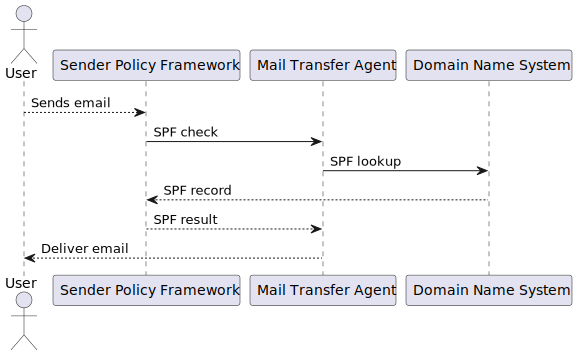
\includegraphics[scale=0.5]{spf.png}
 \end{figure}



 Der Domaininhaber definiert eine SPF-Eintragung im DNS seiner Domain. Diese Eintragung enthält Informationen über die IP-Adressen oder Server, die berechtigt sind, E-Mails im Namen der Domain zu senden. Wenn eine E-Mail gesendet wird, prüft der empfangende Mailserver die SPF-Eintragung der angegebenen Absenderdomain. Der empfangende Mailserver ermittelt die IP-Adresse des sendenden Servers, von dem die E-Mail stammt. Der empfangende Mailserver vergleicht die IP-Adresse mit den in der SPF-Eintragung angegebenen IP-Adressen oder Servern. Wenn die IP-Adresse in der SPF-Eintragung enthalten ist, wird die E-Mail als authentisch eingestuft. Ist die IP-Adresse nicht in der SPF-Eintragung enthalten oder stimmt nicht mit den angegebenen IP-Adressen überein, kann der empfangende Mailserver die E-Mail als verdächtig behandeln und entsprechende Maßnahmen ergreifen, z. B. die E-Mail ablehnen oder in den Spam-Ordner verschieben.
 \subsubsection{DomainKeys Identified Mail - DKIM}
 DKIM fügt der E-Mail eine digitale Signatur hinzu, die mit einem privaten Schlüssel von der Absenderdomain erstellt wurde. Beim Empfang der E-Mail kann der empfangende Mailserver die Signatur überprüfen, indem er den öffentlichen Schlüssel abruft und die Signaturintegrität überprüft. Wenn die Signatur gültig ist, wird die E-Mail als authentisch eingestuft. Die Einrichtung funktioniert wie folgt. Beim Versenden einer E-Mail erstellt der Absender eine digitale Signatur mithilfe eines privaten Schlüssels, der der Absenderdomain zugeordnet ist. Die Signatur wird mit Hilfe einer kryptographischen Hash-Funktion erzeugt, die den Inhalt der E-Mail einschließt. Diese Signatur ist ein eindeutiger Code, der die Echtheit der E-Mail und deren Inhalt bestätigt. Des weiteren veröffentlicht der Absender einen DKIM-Eintrag im DNS seiner Domain. Dieser Eintrag enthält den öffentlichen Schlüssel, der von den Empfängern verwendet wird, um die DKIM-Signatur zu überprüfen. Der Empfangende Mailserver erhält die E-Mail und überprüft, ob die Domain eine DKIM-Signatur besitzt. Ist dies der Fall,  wird der öffentlichen Schlüssel der Absenderdomain aus dem DNS abgerufen. Der empfangende Mailserver verwendet den öffentlichen Schlüssel, um die DKIM-Signatur zu überprüfen. Dabei wird überprüft, ob die Signatur mit dem Inhalt der E-Mail übereinstimmt und ob sie vom korrekten Absender stammt. Wenn die Signatur erfolgreich überprüft wird, wird die E-Mail als authentisch eingestuft.
 \subsubsection{Domain-based Message Authentication, Reporting, and Conformance - DMARC}
 Hierbei handelt es sich um ein weiteren Standard zur E-Mail-Authentifizierung, der SPF und DKIM ergänzt. DMARC ermöglicht es Domaininhabern, Richtlinien festzulegen, wie E-Mails, die nicht den SPF- oder DKIM-Überprüfungen entsprechen, behandelt werden sollen. In der DMARC-Richtlinie kann der Domaininhaber festlegen, wie der empfangende Mailserver mit E-Mails umgehen soll, die nicht den SPF- oder DKIM-Überprüfungen entsprechen. Hierbei stehen verschiedene Optionen zur Verfügung, wie z. B. Ablehnen, Quarantäne oder Überwachen. Wenn der empfangende Mailserver eine E-Mail erhält, die eine DMARC-Richtlinie hat, überprüft er sowohl die SPF- als auch die DKIM-Überprüfung. Der empfangende Mailserver sendet Berichte über die DMARC-Ergebnisse an den Domaininhaber. Diese Berichte enthalten Informationen über die Anzahl der E-Mails, die die SPF- und DKIM-Überprüfungen bestanden oder nicht bestanden haben. Figure 4 zeigt ein DMARC System.
 \begin{figure}[h]
  \caption{DMARC}
  \centering \includegraphics[scale=0.5]{dmarc.png}
 \end{figure}
\newpage
\subsection{Isolierung von Technischen Komponenten}
Eine weitere Möglichkeit das Soziotechnische System Phishing zu behindern, besteht darin technische Komponenten des Nutzers zu isolieren. Durch die Isolation von Anwendungen wie Browser oder Mail Clients wird sichergestellt, dass diese Anwendungen in einer abgeschotteten Umgebung laufen und keinen unbefugten Zugriff auf andere Anwendungen oder sensible Daten haben. Wird die Anwendung dennoch Kompromotiert, sind durch die Isolierung die restlichen Komponenten geschützt. Dies kann auch als Sandboxing bezeichnet werden. Es gibt verschiedene Ansätze zur Isolierung von Anwendungen, wie zum Beispiel Virtuelle Maschienen. Diese sind jedoch schwergewichtig und umständlich einzurichten. Eine elegantere Lösung bietet Container. Mit diesen wird nachfolgend eine Isolierung einer Anwendung durchgeführt. 
\subsubsection{Implementierung einer Anwendungsisolation}
Hierbei wird anhand einer Containerengine wie Docker, die Browseranwendung Firefox isoliert.
Container sind eine leichtgewichtige Art von Virtualisierung auf Betriebssystemebene. Dies kann genutzt werden um eine Anwendung mitsamt ihren Abhängigkeiten als eine abgeschlossene Einheit zu verpacken und zu betrieben.
Dies bietet Vorteile wie Plattformunabhängigkeit und einfache Ausfürbarkeit.
Das Packet aus Anwendung und Abhängigkeiten nennt man auch Container-
Image. Dies kann anhand des Dockerfiles erzeugt werden. Das Dockerfile
enthält alle Instruktionen die zur Erstellung des Images benötigt werden.
\begin{figure}[h]
\caption{Dockerfile }
\begin{shaded}
\begin{internallinenumbers}
FROM ubuntu:14.04

RUN apt-get update \&\& apt-get install -y firefox

RUN export uid=1000 gid=1000 \&\& \

mkdir -p /home/developer \&\& \

echo "developerx\${uid}:\${gid}:Developer,,,:/home/developer:/bin/bash" >> /etc/passwd \&\& \

echo "developerx\${uid}:" >> /etc/group \&\& \

echo "developer ALL=(ALL) NOPASSWD: ALL" > /etc/sudoers.d/developer \&\& \

chmod 0440 /etc/sudoers.d/developer \&\& \

chown \${uid}:\${gid} -R /home/developer

USER developer

ENV HOME /home/developer

CMD /usr/bin/firefox

 \end{internallinenumbers}
\end{shaded}
\end{figure}

Ein Container wird stets auf einem Base Image aufgebaut. Dieses dient als
Fundament für alle folge Instruktionen und enthält je nach Image ein grundlegendes Dateisystem sowie vorinstallierte Software.
In Zeile 1(vgl. Figure 5) wird als Base Image Ubuntu deklariert. Anschließend werden Dienste aktualisiert sowie die Anwendung firefox installiert. Zeile 4-9 dienen der Erstellung eines Benutzers "developer" innerhalb des Containers mit der UID (Benutzer-ID) 1000 und der GID (Gruppen-ID) 1000. Es wird ein Verzeichnis "/home/developer" erstellt und die Berechtigungen und Eigentümerschaft werden entsprechend gesetzt. In Zeile 12 wird festgelegt das beim Start des Containers der Befehl "/usr/bin/firefox" ausgeführt wird, was dazu führt, dass der Firefox-Browser gestartet wird. Mit \colorbox{mshadecolor}{\parbox{0.38\textwidth}{Docker build -t firefox-isolierung .}} wird aus dem Dockerfile ein Image erstellt. Dieses kann nun mit \colorbox{mshadecolor}{\parbox{0.31\textwidth}{Docker run firefox-isloierung}} gestartet werden. Nun öffnet sich der Firefox-Browser auf dem Host-System. Dieser ist allerdings durch den Docker-Container Isoliert.
\section{Soziotechechnische Lösungen}
Soziotechnische Lösungsansätze gegen Phishing stellen einen ganzheitlichen Ansatz dar, der sowohl technische als auch soziale Aspekte berücksichtigt, um Phishing-Angriffe wirksam zu bekämpfen.
Durch die Betrachtung von Phishing als Soziotechnisches System konnten Methoden und techniken herausgearbeitet werden, die Komponenten des Phishing Systems regulieren, sodass dieses stark eingegrenzt ist. Betrachtet man nun das Soziotechnische System, ist festzustellen das viele Interaktionen stark eingegrenzt sind.
\begin{figure}[h]
 \caption{Soziotechechnisches System Phishing nach Maßnahmen}
 \centering \includegraphics[scale=0.5]{iso.png}
\end{figure}

\section{Fazit und Ausblick}
Durch die Betrachtung und Modellierung von Phishing als Soziotechnisches System, konnten Schwachstellen des Systems erkannt und ausgenutzt werden, um Phishingangriffe einzudämmen. Zudem wurdem Soziotechnische Maßnahmen in Form von Kombination von technischen und sozialen Komponenten verwendet um den Schutz zu optmiert. Hierbei wurde darauf abgezielt, Benutzer zu befähigen, Phishing-Angriffe zu erkennen und ihnen aktiv entgegenzutreten, während sie gleichzeitig technische Tools und Sicherheitsmechanismen nutzen, um die Sicherheit der digitalen Kommunikation zu stärken. Durch diese ganzheitliche Herangehensweise können soziotechnische Lösungsansätze einen wichtigen Beitrag zur Reduzierung von Phishing-Angriffen und zum Schutz von Benutzern und Unternehmen leisten.
\newpage
\section{Quellen}
[1] Docker 

[2] Proofpoint
\end{document}
